\documentclass[tikz,border=10pt]{standalone}

\begin{document}

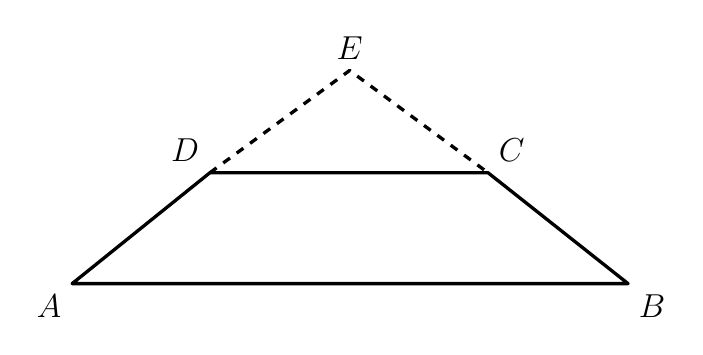
\begin{tikzpicture}[line join=round, line width=1.2pt]
\coordinate (A) at (-3.543,-1.341);
\coordinate (B) at (3.517,-1.341);
\coordinate (C) at (1.739,0.067);
\coordinate (D) at (-1.794,0.067);

  
  
  \coordinate (E) at (-0.019,1.366);

  
  \draw (A) -- (B) -- (C) -- (D) -- cycle;

  
  \draw[dashed] (D) -- (E) -- (C);

  
  \node[font=\fontsize{12}{14.4}\selectfont, below left] at (A) {$A$};
  \node[font=\fontsize{12}{14.4}\selectfont, below right] at (B) {$B$};
  \node[font=\fontsize{12}{14.4}\selectfont, above right] at (C) {$C$};
  \node[font=\fontsize{12}{14.4}\selectfont, above left] at (D) {$D$};
  \node[font=\fontsize{12}{14.4}\selectfont, above] at (E) {$E$};
\end{tikzpicture}
\end{document}